\documentclass[Afour,sageh,times,doublespace]{sagej}
\usepackage[T1]{fontenc}
\usepackage{amsmath,amssymb,amsthm,graphicx,booktabs,url}
\usepackage{xurl}
\usepackage[hidelinks]{hyperref}
\setcitestyle{aysep={,},notesep={: }}
\setcounter{secnumdepth}{2}
\newtheorem{proposition}{Proposition}
\newtheorem{corollary}{Corollary}
\newcommand{\E}{\mathbb{E}}
\newcommand{\Prb}{\mathbb{P}}
\setlength{\tabcolsep}{3pt}
\setlength{\dblfloatsep}{6pt}
\newif\ifreviewcopy
\ifdefined\AnonymousReview\reviewcopytrue\else\reviewcopyfalse\fi
\def\journalname{The European Journal on Artificial Intelligence}
% Submission title: omit unassigned volume, issue, copyright and DOI metadata.
% The official sagej.cls is distributed unchanged.
\makeatletter
\setlength{\@fptop}{0pt}
\setlength{\@fpsep}{14pt}
\setlength{\@fpbot}{0pt plus 1fil}
\setlength{\@dblfptop}{0pt}
\setlength{\@dblfpsep}{6pt}
\setlength{\@dblfpbot}{0pt plus 1fil}
\def\ps@sagepage{%
  \let\@mkboth\@gobbletwo
  \def\@evenhead{\parbox{\textwidth}{\normalsize\sagesf\thepage\hfill\itshape\journalname\\[-6pt]\noindent\rule{\textwidth}{0.25pt}}}%
  \def\@oddhead{\parbox{\textwidth}{\normalsize\sagesf\itshape\leftmark\hfill\thepage\\[-6pt]\noindent\rule{\textwidth}{0.25pt}}}%
  \let\@evenfoot\@empty\let\@oddfoot\@empty}
\def\@maketitle{%
  {\raggedright\titlesize\bfseries\@title\par}
  \bigskip
  {\raggedright\normalsize\bfseries\@author\par}
  \bigskip
  \noindent\usebox\absbox\par
  \medskip\noindent\@keywords\par\bigskip}
\makeatother
\pagestyle{sagepage}
\begin{document}
\ifreviewcopy
\runninghead{Intersectional fairness auditing}
\author{Anonymous review manuscript}
\else
\runninghead{Lu and Wu}
\author{Cenfa Lu\affilnum{1} and Shuda Wu\affilnum{1}}
\affiliation{\affilnum{1}School of Mathematics and Computing Science, Guilin University of Electronic Technology, Guilin, 541004, China.\\
Cenfa Lu: \href{https://orcid.org/0009-0003-3481-3624}{ORCID 0009-0003-3481-3624}; Shuda Wu: \href{https://orcid.org/0009-0003-2590-9608}{ORCID 0009-0003-2590-9608}.}
\corrauth{Cenfa Lu, School of Mathematics and Computing Science, Guilin University of Electronic Technology, Guilin, 541004, China.}
\email{joffin@163.com}
\fi
\title{Model mismatch and missed harms in intersectional fairness auditing: an estimation--detection analysis}
\begin{abstract}
Sharing information across intersectional groups can improve average estimation while obscuring localized harms. We analyze false-negative-rate disparities for a frozen classifier against count-weighted complements. Exact fixed-prior calculations characterize when shrinkage reduces average squared error but suppresses harmful-group screening. A separate finite-sample confirmation procedure combines heterogeneous-reference bounds, binomial tails, and independently weighted Holm testing. Across 60 synthetic configurations with 2,000 repetitions each, the largest observed familywise false-flag frequency was 0.15\% at a nominal 5\% level. Fitted structured-regression and SureMap estimates also reduced average error while suppressing target screens in sparse settings, although raw screens produced substantially more false alerts. Independent weighting sometimes improved confirmation, but the shrinkage-conflict score showed no consistent benefit over raw-disparity weighting. Real-support experiments showed low power for rare targets and favored full-data confirmation for larger targets. These findings distinguish estimation quality, screening sensitivity, and error-controlled audit evidence.
\end{abstract}
\keywords{intersectional fairness, fairness auditing, shrinkage, multiple testing, statistical power}
\maketitle

\section{Introduction}\label{sec:intro}
An audit of a predictive system often has to answer a concrete question: does a particular group experience an unacceptable error rate? The amount of evidence available for that decision can be much smaller than the size of the evaluation dataset. For false-negative-rate (FNR) disparities, the relevant denominator counts positive labels within the group. Intersections of several protected attributes can therefore have very few informative observations even when the overall test set contains thousands of records. Equal-opportunity criteria make this conditional denominator explicit~\citep{hardt2016equality}; subgroup fairness further shows why an overall or marginal comparison can conceal intersectional disadvantage~\citep{kearns2018gerrymandering}.

Information sharing offers a useful response to sparse subgroup estimation. Structured regression (SR) combines attribute-level structure with cell-specific deviations~\citep{herlihy2024structured}; SureMap uses simultaneous mean estimation to improve disaggregated evaluation~\citep{khodak2024suremap}. The estimation objective matters here. An average squared-error improvement need not improve a decision about a particular rare group. A sharing structure that fits most cells can pull an isolated harmful deviation toward a less harmful value. SureMap already explicitly discusses this potential attenuation of disparity and the need for uncertainty assessment~\citep{khodak2024suremap}. Our question is therefore quantitative: how do effective counts, deviation size, shrinkage strength, and confirmation costs jointly determine whether a harmful deviation is reported?

Consider a frozen classifier and an atomic partition fixed before auditing. We compare each group's conditional error rate with the count-weighted error rate of its complement and ask whether their difference exceeds a practical tolerance. Three outputs must remain distinct. A point estimate summarizes performance. A threshold screen applies a decision threshold to that estimate without an error guarantee. A calibrated flag accounts for uncertainty and uses simultaneous testing to support a violation declaration. A screen can be sensitive because it issues many false alerts; a valid test can miss harms because the data are insufficient. Neither output can be assessed by average estimation loss alone.

We investigate this distinction using transparent finite-sample calculations and paired experiments. The theoretical mechanism starts with a fixed Beta shrinker and an oracle reference, where both its squared-error risk and its integer threshold can be computed exactly. This restricted calculation exposes a region in which average estimation improves while the exceptional group's screen is suppressed. This calculation is a diagnostic, rather than a theorem about every fitted empirical Bayes (EB), SR, or SureMap estimator. We then study fitted estimators empirically and construct a separate confirmation protocol for an unknown, possibly heterogeneous complement. Confirmation combines established concentration, nuisance-bound, and multiple-testing ingredients. An independent discovery split may allocate more testing budget to promising groups, but it also reduces the data available for confirmation. A sufficient-bound calculation makes this cost explicit.

We analyze estimation and audit decisions under a common target and data budget. We give exact fixed-prior decision boundaries; evaluate how fitted sharing methods behave in prespecified isolated-deviation and structural controls; and compare independently weighted confirmation with full-data testing, retaining negative comparisons. The results support a limited but practically relevant conclusion: an estimator selected for lower average loss is not, by that fact alone, a more reliable harm detector. Additional modeling of estimation uncertainty and the audit's decision objective remains necessary. The study does not propose a fairness test that is universally better.

\section{Related work}\label{sec:related}
\subsection{Sharing information in disaggregated evaluation}
Bayesian intersectional modeling quantifies uncertainty while borrowing information across groups~\citep{foulds2020bayesian}. Model-based metrics also improve sample efficiency for subpopulation performance estimation~\citep{miller2021modelbased}, and Bayesian inference has been used when fairness measurements involve unlabeled data~\citep{ji2020trust}. These approaches motivate examining how model assumptions interact with the downstream audit decision. Bashir's discussion of intersectional multilevel analysis emphasizes that pooling can affect the interpretation of small groups~\citep{bashir2026reweighting}. That setting differs from our frozen-classifier error audit, but reinforces the distinction between average modeling performance and a specific intersectional estimand.

SR uses inverse-variance weighted Lasso with an unpenalized intercept and structural and cell-specific terms~\citep{herlihy2024structured,tibshirani1996lasso}. Its original inference uses residual bootstrap Lasso plus partial ridge (rBLPR) machinery~\citep{herlihy2024structured,liu2020bootstrap}. We implement a clearly labeled adapter for point estimation; we do not implement those intervals. Since its saturated identity terms can represent an arbitrary cell vector, an isolated deviation is not necessarily excluded from its model class. Here, \emph{model mismatch} means a departure from the sharing structure encouraged by regularization or pooling; attenuation can arise through regularization even in a saturated class. SureMap provides a more recent mean-estimation comparator~\citep{khodak2024suremap}. Its earlier qualitative warning includes the possibility of optimistic disparity estimates. Our fixed-Beta calculation quantifies a restricted version of that mechanism; it does not establish failure of SureMap's uncertainty procedures.

\subsection{Statistical evidence for fairness violations}
Cherian and Cand\`es develop bootstrap-based fairness audits with asymptotic simultaneous certification guarantees and false-discovery-rate control for flagging under their stated conditions~\citep{cherian2024statistical}. Their framework shows why uncertainty and multiplicity are central to auditing. Size-adaptive fairness testing (SAFT) uses asymptotic inference for larger groups and Dirichlet--multinomial posterior inference for smaller groups~\citep{ferrara2025saft}. Single-cell posterior smoothing is different from cross-group shrinkage, and posterior tail probabilities should not automatically be interpreted as frequentist p-values. We include a local conditional Dirichlet mean as a point diagnostic, not a reproduction of the complete SAFT procedure. Our analysis does not reproduce the original SR intervals or Cherian--Cand\`es bootstrap decisions. An exploratory interval analysis implements the published SAFT interval ingredients with an explicit adaptation for conditional FNR; its tolerance rule is distinct from the original two-sided zero-parity test. The empirical claims concern the implemented estimators, intervals, and confirmation rules.

FairCert combines Clopper--Pearson intervals with Bonferroni correction for finite-sample bounds on between-group false-positive-rate and true-positive-rate gaps~\citep{sikder2026faircert}. Our exact-binomial comparator projects a simultaneous rate rectangle onto count-weighted group--complement FNR contrasts and uses a lower endpoint above tolerance to declare a violation.

The preprint by \citet{tang2026tolerance} (version 1, 1 October 2026) distinguishes tolerance-based violation certification from sensitivity-oriented screening using empirical likelihood. Its asymptotic calibration and reference assumptions differ from the fixed-count heterogeneous-complement construction here. We do not claim to introduce tolerance-based fairness auditing or the distinction between false declarations and missed violations.

\subsection{Independent weighting and confirmation}
Holm's sequential correction and weighted multiple-testing procedures provide established familywise error control~\citep{holm1979simple,kang2009weighted}. Learning testing weights on an independent sample is also established~\citep{rubin2006splitting}; cross-weighting provides additional formulations under its independence conditions~\citep{ignatiadis2021covariate}. Our split separates individuals within every atomic stratum. It does not assume that fairness hypotheses with shared complements are independent. The confirmation p-value combines a Hoeffding reference bound~\citep{hoeffding1963probability} with a binomial target tail, using a nuisance-bound principle related to Berger and Boos~\citep{berger1994pvalues}. These are conventional statistical ingredients. The substantive comparisons examine when prioritization provides enough testing budget to offset the cost of splitting, and whether priorities informed by shrinkage offer an improvement over priorities based on raw disparities.

\section{Audit target and sampling design}\label{sec:audit-target}

We audit a frozen binary classifier, including its decision threshold, on a
prespecified finite family of $G$ mutually exclusive intersectional cells.
Write $E=\mathbf{1}\{f(X)=0\}$ for a classification error among observations
with true label $Y=1$. The classifier's false-negative rate (FNR) in cell $g$
is $p_g=\Pr(E=1\mid Y=1,g)$. Its effective sample size $n_g$ counts
positive-label observations, rather than all cell members. Our target is a
one-sided difference relative to the count-weighted complement, with a fixed
practical tolerance $0<\Delta<1$.

In the fixed-stratum design, positive counts $n_1,\ldots,n_G$ are fixed and
errors are independent Bernoulli observations with constant rate $p_g$
within each cell. Let $N=\sum_h n_h$, $\pi_g=n_g/N$, and assume
$1-\pi_g>0$ so that a reference exists. Define
\begin{equation}
 \begin{aligned}
 q_g&=\sum_{h\ne g}\frac{\pi_h}{1-\pi_g}p_h,\\
 \delta_g&=p_g-q_g,\qquad H_{0g}:\delta_g\le\Delta.
 \end{aligned}
 \label{eq:theory-target}
\end{equation}
Although the target error count is binomial, the complement count generally
has a Poisson-binomial law. With $\bar p=\sum_h\pi_hp_h$, the equivalent
identity $\delta_g=(p_g-\bar p)/(1-\pi_g)$ also shows that an injected
increase in $p_g$ need not equal the resulting disparity. We use the actual
$\delta_g$ to identify harmed cells.

In an independent and identically distributed (IID) population audit, the same
comparison has a different interpretation: $q_g=\Pr(E=1\mid Y=1,g^c)$. Conditional on the two positive
counts for a fixed cell, the target and complement counts are independent
binomials. Our fixed-count simulations instead use
Eq.~\eqref{eq:theory-target}; a binomial reference assumption is unnecessary
for their confirmation test. Neither model automatically describes
dependent patients, households, or complex survey sampling.

Let $\mathcal H=\{g:\delta_g>\Delta\}$. For audit flags $F_g\in\{0,1\}$,
the familywise error rate (FWER) is
$\Pr\{\exists g\notin\mathcal H:F_g=1\}$. The audit missed-harm rate is
\begin{equation}
 \mathrm{MHR}=\frac{1}{|\mathcal H|}
      \sum_{g\in\mathcal H}\Pr(F_g=0), \qquad |\mathcal H|>0.
 \label{eq:theory-mhr}
\end{equation}
Thus, MHR concerns audit non-detection, whereas classifier FNR concerns
prediction errors. MHR is undefined when no cell is harmed. On a fully
supported design, estimation is assessed separately through macro risk
$G^{-1}\sum_g\mathbb E(\widehat p_g-p_g)^2$ and prevalence-weighted risk
$\sum_g\pi_g\mathbb E(\widehat p_g-p_g)^2$. These averages do not specify
the probability of identifying a particular harmed cell.

Splitting must preserve the target. We assign independent error
observations to discovery $D$ and confirmation $C$, with
$n_h^C=c n_h$ exactly in every supported cell, $0<c<1$, and integer counts in both
parts. Then complement proportions, and hence $q_g$, are unchanged.
Random within-cell split counts generally change the conditional
complement weights. Such a design requires an explicitly standardized
reference instead. A zero target or reference count is recorded as
insufficient information, with a confirmation p-value of one; the cell remains
in the registered family. Non-rejection is inconclusive and does not
certify fairness.

\section{Estimation and screening can separate}\label{sec:separation}

Sharing information across cells can improve mean estimation, as pursued
by structured regression and SureMap~\citep{herlihy2024structured,khodak2024suremap}. To isolate the decision
mechanism, we first examine a fixed Beta posterior mean. This calculation
does not characterize all fitted empirical Bayes, structured regression,
or SureMap estimators. Its reference is known, and its threshold decision
is a descriptive screen rather than an error-controlled test.

\begin{proposition}[Fixed-prior risk and strict-screen boundary]
\label{prop:theory-shrinkage}
Let $X\sim\mathrm{Bin}(n,p)$, $n\ge1$, and fix $\kappa>0$ and
$\mu\in(0,1)$ independently of $X$. Set
$\widehat p=X/n$ and $\widetilde p=(X+\kappa\mu)/(n+\kappa)$.
For an oracle reference $r$, let $t=r+\Delta\in(0,1)$ and define
$A_0=\{\widehat p>t\}$ and $A_\kappa=\{\widetilde p>t\}$.
Writing $R_\kappa(p)=\mathbb E(\widetilde p-p)^2$ and
$R_0(p)=p(1-p)/n$, we have
\begin{equation}
 \begin{aligned}
 &R_\kappa(p)-R_0(p)\\
 &\quad=\frac{\kappa^2(p-\mu)^2-(2\kappa+\kappa^2/n)p(1-p)}
 {(n+\kappa)^2}.
 \end{aligned}
 \label{eq:theory-risk}
\end{equation}
Moreover,
\begin{equation}
 \begin{aligned}
 \Pr_p(A_\kappa)&=\Pr_p(X\ge K_\kappa),\\
 K_\kappa&=\lfloor nt+\kappa(t-\mu)\rfloor+1,
 \end{aligned}
 \label{eq:theory-cutoff}
\end{equation}
where $K_\kappa\le0$ or $K_\kappa>n$ gives probability one or zero,
respectively. If $t>\mu$, the integer cutoff cannot decrease. If
\begin{equation}
 \kappa(t-\mu)\ge n(1-t),
 \label{eq:theory-collapse}
\end{equation}
the shrunk screen never selects the cell. If $p=t+\varepsilon\le1$,
$\varepsilon>0$, and $a=\kappa(t-\mu)-n\varepsilon>0$, then
\begin{equation}
 \begin{aligned}
 \Pr_p(A_\kappa)&\le e^{-2a^2/n},\\
 \Pr_p(A_0^c)&\le e^{-2n\varepsilon^2}.
 \end{aligned}
 \label{eq:theory-screen-bound}
\end{equation}
\end{proposition}

Equation~\eqref{eq:theory-risk} balances variance reduction against bias;
Eq.~\eqref{eq:theory-cutoff} tracks the error count needed to cross a
decision threshold. Their joint dependence on effective count, tolerance,
signal, and shrinkage matters. For $t>\mu$, the dimensionless ratio
$\kappa(t-\mu)/(n\varepsilon)>1$ means that shrinkage raises the threshold
above the harmed cell's expected error count. This is a finite-sample
diagnostic, not a minimax phase transition. The integer cutoff may remain
unchanged after a small increase in the real threshold.

An exact example illustrates this separation. Take five equally sized
cells with $n=10$, four with rate $0.1$ and one with rate $0.35$, and fix
$\mu=0.1$, $\kappa=90$, and $\Delta=0.1$. The exceptional cell's complement
has rate $r=0.1$, so its oracle threshold is $t=0.2$. Macro mean squared error (MSE) is
$0.01175$ for raw proportions and $0.0102425$ for shrinkage. The raw
screen selects this cell with probability
$\Pr_{0.35}\{X\ge3\}=0.7383926086$, while the shrunk screen would require
$X>11$ and has selection probability zero. These numbers follow from
finite-binomial calculations rather than fitted experiment outcomes. The
prior is deliberately strong; whether fitted methods reach a comparable
regime is an empirical question.

More generally, each cell with $p=\mu$ has strictly smaller risk under
this shrinker. Sufficiently many such cells offset the finite risk cost of
one exceptional cell, even when its screen collapses. The calculation
holds conditionally for hyperparameters learned from independent data.
Treating hyperparameters fitted to the same data as fixed would not justify
Eq.~\eqref{eq:theory-risk}. Full proofs appear in
Appendix~\ref{app:theory-proofs}.

\section{Confirmation and allocation under a common budget}
\label{sec:confirmation}

\subsection{Unknown-reference confirmation}

Our primary confirmation engine combines a Hoeffding upper bound for the
reference with an exact binomial target tail; we refer to it as HB. The
ingredients are established concentration and nuisance-parameter
methods~\citep{hoeffding1963probability,berger1994pvalues}.

\begin{proposition}[HB p-value with a heterogeneous reference]
\label{prop:theory-hb}
Let $X\sim\mathrm{Bin}(n,p)$, $n\ge1$. Let the reference observations
$B_1,\ldots,B_m$, $m\ge1$, be independent Bernoulli variables with
possibly unequal means $q_1,\ldots,q_m$. Define
$q=m^{-1}\sum_jq_j$ and $\widehat q=m^{-1}\sum_j B_j$.
Fix $0<\eta<1$ before observing confirmation outcomes, and set
\begin{equation}
 \begin{aligned}
 U_q&=\min\left\{1,\widehat q+
          \sqrt{\frac{\log(1/\eta)}{2m}}\right\},\\
 \theta_U&=\min\{1,U_q+\Delta\}.
 \end{aligned}
 \label{eq:theory-upper-reference}
\end{equation}
\begin{equation}
 \begin{aligned}
 P_{\mathrm{HB}}&=\min\{1,\eta+T_{\theta_U}(X)\},\\
 T_\theta(x)&=\Pr\{\mathrm{Bin}(n,\theta)\ge x\}.
 \end{aligned}
 \label{eq:theory-hb}
\end{equation}
Under $p-q\le\Delta$, $\Pr(P_{\mathrm{HB}}\le u)\le u$ for all
$u\in[0,1]$. Setting $P_{\mathrm{HB}}=1$ when either denominator is zero
preserves validity.
\end{proposition}

The binomial target assumption is essential: an atomic cell has a common
rate, whereas an aggregate of heterogeneous cells need not. The proof
allows a heterogeneous complement and does not replace its law by a
binomial approximation. For a fixed standardized reference
$q=\sum_h\nu_hp_h$, with fixed $\nu_h\ge0$ and $\sum_h\nu_h=1$,
samples from supported cells instead give
$\widehat q=\sum_h\nu_h\widehat p_h$ and upper radius
$\{\frac12\log(1/\eta)\sum_h\nu_h^2/n_h\}^{1/2}$.
Unsupported cells with positive reference weight require a worst-case
contribution or an insufficient-information outcome.

For heterogeneous targets, a separate valid alternative uses independent
Bernoulli observations on both sides. With empirical difference $d$ and
$V=1/n+1/m$, the difference-Hoeffding p-value is
\begin{equation}
 \begin{aligned}
 P_{\mathrm H}&=\exp\{-2(d-\Delta)_+^2/V\},\\
 (x)_+&=\max\{x,0\}.
 \end{aligned}
 \label{eq:theory-hoeffding}
\end{equation}
It tests the difference of the two average means. We use its conservative
boundary for planning below; it does not supply a power formula for HB.

\subsection{Independent discovery weights and weighted Holm}

Discovery chooses nonnegative scores $s_g(D)$ without using confirmation
outcomes. For a fixed floor $0<\rho\le1$, define
\begin{equation}
 w_g=\frac{\rho}{G}+(1-\rho)\frac{s_g}{\sum_hs_h},
 \label{eq:theory-weights}
\end{equation}
using $w_g=1/G$ when all scores vanish. Thus $w_g\ge\rho/G$ and
$\sum_gw_g=1$. Independent weighting and sample splitting are established
multiple-testing tools~\citep{kang2009weighted,rubin2006splitting}; here
their role is to allocate a fixed audit budget.

\begin{proposition}[Conditional strong FWER control]
\label{prop:theory-holm}
Fix $0<\alpha<1$. Suppose the confirmation p-values for true nulls are super-uniform conditional on
discovery and the legitimate confirmation design. Order hypotheses by
$P_g/w_g$, with a fixed rule for ties, and reject sequentially while
\begin{equation}
 P_{(j)}\le\frac{\alpha w_{(j)}}{\sum_{k=j}^G w_{(k)}},
 \label{eq:theory-holm}
\end{equation}
stopping at the first failure. Then FWER is at most $\alpha$, allowing
arbitrary dependence among confirmation p-values. The rejection set
contains every weighted-Bonferroni rejection $P_g\le\alpha w_g$.
\end{proposition}

The proof is the usual first-false-rejection argument for step-down
testing~\citep{holm1979simple}. Misspecified discovery scores affect
allocation, while conditional validity provides error control. The floor
ensures a positive minimum testing budget; it gives neither equal power
nor equal information.

The five score options are equal scores, $\sqrt{n_g^D}$, raw excess
$(\widehat\delta_g^D-\Delta)_+$, empirical Bayes excess
$(\widetilde\delta_g^D-\Delta)_+$, and a conflict score
\begin{equation}
 \begin{aligned}
 s_g^{\mathrm{conflict}}&=(\widehat\delta_g^D-\Delta)_+\\
 &\quad+(\widehat\delta_g^D-\widetilde\delta_g^D)_+.
 \end{aligned}
 \label{eq:theory-conflict}
\end{equation}
Raw and fitted differences use their respective count-weighted
complements. Scores are zero for cells without discovery observations.
The conflict score is a baseline option for testing whether disagreement
helps allocation; a consistent additional benefit has not been demonstrated, and the score is not
presented as a new testing principle.

The primary comparator uses all audit observations with HB and ordinary
Holm, corresponding to equal weights. The split methods use the same total
count budget, estimand, and p-value engine. To isolate floor effects, all
main comparisons and floor ablations fix
$\eta=\alpha\rho_{\min}/(20G)$ with $\rho_{\min}=0.05$, rather than changing
the HB engine with $\rho$. For planned floors $\rho\ge\rho_{\min}$,
$\eta\le\alpha w_g/20$. Score definitions, floors, and nuisance budgets
are frozen before confirmation.

\subsection{The allocation advantage must offset splitting}

For supported confirmation counts, let $V_g=1/n_g^C+1/m_g^C$.
For Eq.~\eqref{eq:theory-hoeffding}, define the sufficient boundary
$b_g(w)=\{(V_g/2)\log[1/(\alpha w)]\}^{1/2}$. If
$\delta_g=\Delta+\varepsilon_g$ and $\varepsilon_g>b_g(w_g)$,
weighted Holm has conditional power at least
\begin{equation}
 1-\exp\{-2[\varepsilon_g-b_g(w_g)]^2/V_g\}.
 \label{eq:theory-power-envelope}
\end{equation}
Below that boundary the stated lower bound is zero, which says nothing
about whether actual power is zero. Replacing $w_g$ by $\rho/G$ gives a
score-independent version.

\begin{corollary}[Comparison of Hoeffding sufficient boundaries]
\label{cor:theory-split}
Suppose confirmation retains exactly a fraction $c$ of each relevant count,
so $V_C=V_A/c$, where $A$ denotes all audit data. The split
weighted-Bonferroni sufficient boundary is strictly smaller than the
full-data equal-weight Bonferroni boundary if and only if
\begin{equation}
 w_g>\alpha^{c-1}G^{-c}.
 \label{eq:theory-split-cost}
\end{equation}
\end{corollary}

At $\alpha=0.05$ and $c=0.5$, this requires $w_g>0.5590$ for $G=64$,
and $w_g>1.1180$ for $G=16$. The latter is impossible. These are
comparisons of conservative sufficient boundaries, not an ordering of
actual powers, and do not compare split and full-data Holm directly.
Full-data Holm can improve upon its Bonferroni counterpart. Consequently,
the FWER guarantee provides no general power advantage for splitting;
that question requires the paired empirical comparisons.


\section{Experimental design}\label{sec:experiments}
\subsection{Paired synthetic audit datasets}
We fix the group counts before generating errors. The main grid has $G\in\{16,32,64\}$, an exceptional cell with a positive count $n_*\in\{10,20,40,80,160\}$, and other cell counts cycling through $10,20,40,80,160,320$. Ordinary cells have error probability .12. In the 45 sparse-deviation configurations, the exceptional probability is $.12+.05+\varepsilon$, with $\varepsilon\in\{.10,.20,.30\}$. Because all its complement cells have probability .12, its true disparity is exactly $.05+\varepsilon$. Null and harmed labels for \emph{all} cells are computed from the true count-weighted complement, rather than from the injected increment alone.

Five additional controls for each $G$ produce 60 main configurations: a homogeneous global null; a boundary null with exceptional probability .17; harm placed in a count-320 cell; multiple harmful cells with probability .37; and additive probabilities $.08+.035a_1+.02a_2+.015a_3$, where $a_1=i\bmod2$, $a_2=\lfloor i/2\rfloor\bmod4$, and $a_3=\lfloor i/8\rfloor\bmod4$ for zero-indexed cell $i$. The last configuration is a main-effects control. The synthetic attribute tuples used by SR and SureMap are $(i\bmod2,\lfloor i/2\rfloor\bmod4,\lfloor i/8\rfloor)$; in the 64-cell additive control, the generating effect for the third attribute repeats across its categories.

Each main configuration has 2,000 repetitions. We generate independent discovery and confirmation errors at the same probability within each group, with a confirmation fraction $c=.8$. The full-data counts are their sum, providing an identical total data budget and paired outcomes. Counts are multiples of ten, so all registered split fractions preserve complement proportions exactly. We use $\Delta=.05$, nominal $\alpha=.05$, floor $\rho=.1$, and fixed $\eta=\alpha(.05)/(20G)$. The latter remains unchanged when the floor is ablated. Full-data HB plus Holm is the primary calibrated comparator; full-data difference-Hoeffding plus Holm is a validity/conservatism ablation. The split procedures with uniform, size, raw, EB, and conflict scores use the same HB confirmation engine. No oracle harm labels enter a discovery score.

The split ablation uses $G=32$, $n_*\in\{20,80\}$, exceptional probability .37, $c\in\{.5,.8,.9\}$, and $\rho\in\{.05,.1,.5,1\}$, giving 24 configurations with 1,000 repetitions each. We retain every prespecified combination rather than select a favorable split or random seed. The fixed-prior analytic sensitivity calculation separately evaluates concentrations $0,1,5,20,90,100,500$. It does not provide empirical evidence from an estimator with a fitted prior.

\subsection{Point estimators and implementation scope}
The basic estimators are raw cell proportions, complete pooling, a fixed Beta mean centered at .12 with concentration 100, equal-group moment EB, and the conditional group mean $(K_g+1)/(n_g+2)$ from a counts-plus-one four-cell Dirichlet model. Applying this last mean to every atomic cell and forming its weighted complement is a local plug-in diagnostic, not the native two-group SAFT audit.

For moment EB, the center is the mean of nonempty raw cell rates, clipped to $[10^{-4},1-10^{-4}]$. We subtract the mean estimated binomial sampling variance $\widehat p_g(1-\widehat p_g)/\max(n_g-1,1)$ from the mean squared deviation across cells, floor the result at $10^{-8}$, and set the concentration to $\mu(1-\mu)/\widehat\tau^2-1$, clipped to $[2,2000]$. This fully specified local estimator is not SR, SAFT, or a fixed independent prior. Its hyperparameters are fitted to all the data, which is outside the scope of the fixed-prior theorem.

The SR point adapter minimizes a count-weighted squared-error loss with an unpenalized intercept, attribute indicators, all cell-identity indicators, and an $\ell_1$ penalty. The common variance factor is absorbed into the penalty scale. Group-stratified five-fold cross-validation at the individual level selects among a zero-penalty fit and 32 geometrically spaced positive penalties from $10^{-4}\alpha_{\max}$ to $\alpha_{\max}$. This differs from the original ten-fold specification. No probability clipping, auxiliary model covariates, or original rBLPR intervals are added. The zero-penalty saturated fit is included, allowing cross-validation to choose raw interpolation.

SureMap uses the authors' MIT-licensed single-task numerical implementation, revision \texttt{ccd80ae}, applied to literal Bernoulli error arrays reconstructed from sufficient counts. The import bridge retains the estimator and data-statistics function bodies, removes unused heavyweight imports and an optional just-in-time (JIT) decorator, and checks the two source-file hashes. This is an import adaptation, not a reproduction of the complete upstream environment. Failed or nonfinite outputs are recorded rather than replaced by another estimator. All paired baselines returned finite outputs in the reported subsets. A stricter follow-up analysis of all 28 synthetic SR paths with warnings preserved the selected penalties and screening conclusions; the reconstruction and tolerances are reported in Appendix~\ref{app:inventory}.

We compare these point estimators on the first 120 repetitions of seven prespecified $G=32$ synthetic settings: four sparse combinations $(n_*,\varepsilon)\in\{20,80\}\times\{.10,.30\}$ and the homogeneous-null, common-harm, and additive controls. Macro MSE and exceptional-cell MSE assess different estimation objectives. The plug-in screen is $\widehat p_g-\widehat q_{-g}>.05$; it has no frequentist error guarantee. Its rate is reported separately from calibrated flagging power.

\subsection{Exploratory interval diagnostics on retained outcomes}
An exploratory analysis, specified after the primary experiments, reuses the first 120 repetitions of all seven point-comparison settings. It does not generate any additional audit outcomes or classifier fits. We compare unadjusted 95\% Wald contrast intervals, a local conditional-FNR implementation of SAFT's published interval construction~\citep{ferrara2025saft}, and a classical simultaneous exact-binomial baseline~\citep{clopper1934confidence}. The Wald interval uses the raw target--complement difference and the plug-in variance $\widehat p_g(1-\widehat p_g)/n_g+\widehat q_g(1-\widehat q_g)/n_{-g}$.

For the SAFT construction, Algorithm~1 switches to Wald only when all four outcome-by-membership counts, $K_g,n_g-K_g,K_{-g},n_{-g}-K_{-g}$, are at least 30. Otherwise a counts-plus-one Dirichlet posterior is used. Its two conditional rates are independent Beta variables, so we sample their difference directly, using 10,000 draws and inverse empirical quantiles at .025 and .975. Conditioning on $Y=1$ and treating an error as the binary outcome maps the contrast to FNR. The known fixed-stratum reference may be heterogeneous, so the aggregated posterior remains a working model whose coverage is evaluated rather than assumed. Using the lower endpoint $>.05$ is a local one-sided tolerance rule, not the original two-sided zero-parity decision, and has no claimed FWER guarantee.

The simultaneous baseline forms two-sided Clopper--Pearson rate intervals $[L_h,U_h]$ with noncoverage at most $\alpha/G$ for each cell, then uses $[L_g-\sum_{h\ne g}n_hU_h/n_{-g},\ U_g-\sum_{h\ne g}n_hL_h/n_{-g}]$ for each contrast. By a union bound, all rate intervals cover their true rates with probability at least $1-\alpha$. On that event, the nonnegative complement weights ensure that every true contrast lies within its interval. Thus its lower-endpoint tolerance decisions control familywise false declarations under the group-binomial assumptions, without requiring a binomial heterogeneous complement. This is a conventional conservative benchmark, not a proposed method.

We retain target and whole-family coverage, interval widths, tolerance-rule frequencies, and simulation MCSEs for every setting. The pointwise and simultaneous intervals have different error targets and cannot establish matched-FWER power rankings. A second posterior seed repeats the first 20 datasets in each setting to expose numerical Monte Carlo sensitivity. Native two-sided zero-parity behavior is reported separately for the homogeneous global null. An exploratory first implementation used an incorrect total-count switch; it was superseded before manuscript use by the four-count implementation and remains labelled separately in the archive.

\subsection{Public-data support and frozen classifiers}
We prepare Adult, Diabetes 130-US Hospitals, and the 2018 Alabama American Community Survey (ACS) Income and Employment tasks. The ACS tasks come from the Folktables framework~\citep{ding2021retiring}. We use the task definitions in version 0.0.12 (\url{https://pypi.org/project/folktables/0.0.12/}). The Diabetes source concerns hospital readmission data~\citep{strack2014impact}. Official raw archives, hashes, target definitions, row identifiers, and all transformations accompany the code. Adult combines its supplied train/test files and uses a new seeded split; original person identifiers are unavailable. Diabetes retains the minimum encounter identifier per patient, then uniformly caps the eligible patient sample at 50,000 without label-based sampling. This identifier rule is deterministic, not verified clinical chronology. Readmission within 30 days is the positive label; features include information available by discharge, and no prospective clinical effectiveness is claimed.

Each task uses an approximately 60/20/20 split into training, calibration, and audit sets. Diabetes splits distinct patients, ACS splits households by \texttt{SERIALNO}, and Adult splits record identifiers. Folktables' \texttt{ACSEmployment} task retains all ages, whereas Ding et al.~\citep{ding2021retiring} describe ages 16--90. ACS Income uses the package's adult filter. The ACS tasks share source people and are not independent populations. No survey weights are used. Household separation prevents train leakage across households, but does not remove dependence among records within the audit split.

Groups are sex $\times$ source race category $\times$ age band ($<40$, 40--69, $70+$). Source race categories are retained rather than pooled across datasets; missing categories receive their own level. We retain the full Cartesian universe, including empty cells. Logistic regression (LR) and histogram gradient boosting (HGB) exclude these protected fields but retain other potential proxies. Their preprocessing is fitted only on training data. LR uses standardized numerical variables, one-hot-encoded categorical variables, $C=1$, and at most 400 iterations. HGB uses imputation and categorical encoding fitted on the training data, 100 iterations, learning rate .08, at most 15 leaves and depth 5, minimum leaf size 30, and $\ell_2$ regularization 1, with early stopping disabled. A single threshold for each model is selected from scores for calibration positives to give an empirical calibration FNR at most .2, with threshold ties predicted positive. Predictions are then frozen.

Table~\ref{tab:data} reports support on the original audit sets. Omitting protected inputs does not guarantee fairness. Original-data rates and model AUCs are descriptive sample facts; no exact binomial population inference is asserted for these observational records. In particular, ACS survey design and within-household dependence do not satisfy the independent-error model by assumption.
% Generated by src/make_tables.py; source analysis/*.csv and retained results.
\begin{table*}[t]
\centering\small
\caption{Original-data support and discrimination on the frozen audit split. Effective audit counts $N^+_A$ record the number of positive labels; empty cells remain registered. The area under the receiver operating characteristic curve (AUC) is descriptive and does not establish fairness.}\label{tab:data}
\begin{tabular}{lrrrrrrr}
\toprule
Task & Used $N$ & $N^+_A$ & $G$ & $n_g>0$ & $n_g=0$ & $0<n_g<10$ & AUC LR/HGB \\
\midrule
Adult & 48,842 & 2,338 & 30 & 22 & 8 & 10 & 0.902/0.918 \\
Diabetes & 50,000 & 876 & 54 & 29 & 25 & 19 & 0.654/0.653 \\
ACS Income & 22,268 & 1,347 & 54 & 23 & 31 & 12 & 0.851/0.832 \\
ACS Employment & 47,777 & 3,922 & 54 & 35 & 19 & 16 & 0.836/0.839 \\
\bottomrule
\end{tabular}
\end{table*}


\subsection{Known-truth real-support experiments}
For each task we retain cells with at least ten audit positives and five calibration positives. We round audit counts down to multiples of ten and cap them at 1,000. This leaves 11/30 Adult cells, 10/54 Diabetes cells, 10/54 Income cells, and 19/54 Employment cells. The complement in these experiments is explicitly defined over this \emph{selected family with capped and rounded counts}, not the original complete partition. Cells excluded by this benchmark rule are not certified fair; their original support remains reported in Table~\ref{tab:data} and the accompanying group table.

Calibration error counts define a fixed template $p_g=(K_g^{\rm cal}+.5)/(n_g^{\rm cal}+1)$, clipped to $[.02,.8]$. One geometry retains these heterogeneous rates; the other assigns their count-weighted mean to ordinary cells. The smallest selected cell is the target, with fixed probability equal to its template complement plus .25, capped at .95. The cap is inactive for the reported targets. Actual truth is recomputed from the final vector. Every selected target has $n_*=10$ and $\delta_*=.25$. Independent Bernoulli errors generated from these fixed vectors give known truth conditional on the templates. They do not establish real population truth or preserve dependence in the real errors.

There are 16 configurations: four tasks, two classifiers, and two geometries, each with 1,000 repetitions. SR and SureMap are evaluated on the first 80 repetitions of the eight heterogeneous configurations. These templates provide sensitivity to realistic support and baseline-rate patterns, but not a general robustness claim across all rare-cell sizes, harm strengths, or survey designs.

\subsection{Metrics, uncertainty, and reproducibility}
We additionally freeze a 32-configuration analysis of sensitivity to support before generating its outcomes: four tasks, two classifiers, capped versus uncapped rounded counts, and two deterministic target rules. Eligibility and calibration-heterogeneous templates remain fixed. The first rule selects the smallest eligible cell; the second selects the smallest cell with at least 80 transformed positives, using original group order to break ties. The resulting larger counts are 140 for Adult, 130 for Diabetes, 170 for Income, and 130 for Employment. Every target's probability is set to its own transformed complement rate plus .25. We retain 1,000 repetitions with independent SeedSequence child streams of seed 20261024. Only Adult has a group count above the 1,000 cap; other tasks retain the prespecified identical C/U templates as independent simulation repeats. Comparisons with larger targets change both cell identity and support, rather than isolating the causal effect of increasing the count for one fixed cell.

Familywise error rate (FWER) is the probability of at least one flag among the cells whose true disparity is at most $\Delta$. Target power is the flag probability of the designated harmed cell; its missed-harm rate is one minus that probability. Macro MSE weights cells equally; prevalence-weighted MSE weights by the positive counts. Retained arrays also support mean and worst harmed-cell power. No fairness-certification procedure is implemented: a nonflag is inconclusive.

For repetition-level quantities, Monte Carlo (MC) standard errors (MCSEs) are sample standard deviations divided by the square root of the number of repetitions. Power differences use the within-repetition difference, preserving pairing. Plot bars are $1.96$ MCSE unless otherwise stated. These summaries describe simulation error; they are not uncertainty intervals for an original population's fairness. Wilson intervals~\citep{wilson1927probable} remain informative when zero false flags are observed. The reported maxima are selected across the fixed grid; their pointwise intervals are not simultaneous confidence bounds. Counts of grid-level wins are descriptive, not multiplicity-adjusted tests of dominance. With 120 repetitions, pointwise 95\% Wilson intervals for probabilities observed as 0/120 and 120/120 are [0, .0310] and [.9690, 1], respectively; zero sample MCSE does not remove this simulation uncertainty. Displayed decimals use round-to-nearest formatting with ties to even, and unrounded values remain in the machine-readable outputs.

The main random seed is 20261022, with independent SeedSequence child streams by configuration; extended runs use seed 20261023 and a deterministic sequential generator. We retain generated counts, probabilities, weights, estimates, decisions, scenario definitions, and run-time/source-hash metadata. All computations use CPU only. Figures were generated with Matplotlib and exported as vector PDFs.

\ifreviewcopy
\textbf{Computational assistance.} OpenAI Codex assisted with literature retrieval, code development and checking, statistical derivation, analysis, figure preparation, and manuscript drafting and editing. The authors retain responsibility for the scientific claims, verification of results, and final text.
\else\fi

\section{Results}\label{sec:results}
\subsection{Lower estimation risk can coexist with suppressed screens}
Figure~\ref{fig:exact} displays the exact fixed-prior calculation. With five count-ten cells, four ordinary rates .1, one exceptional rate .35, center .1, oracle reference .1, and tolerance .1, concentration 90 reduces macro MSE from .01175 to .0102425. The exceptional-cell raw screen probability is .7383926086; the shrunk screen probability is zero. These numbers follow from finite-binomial risks and tails, without Monte Carlo error. The deliberately strong fixed prior illustrates existence and the decision boundary; it is not an estimate of the strength selected by SR or SureMap.
\begin{figure*}[t]\centering
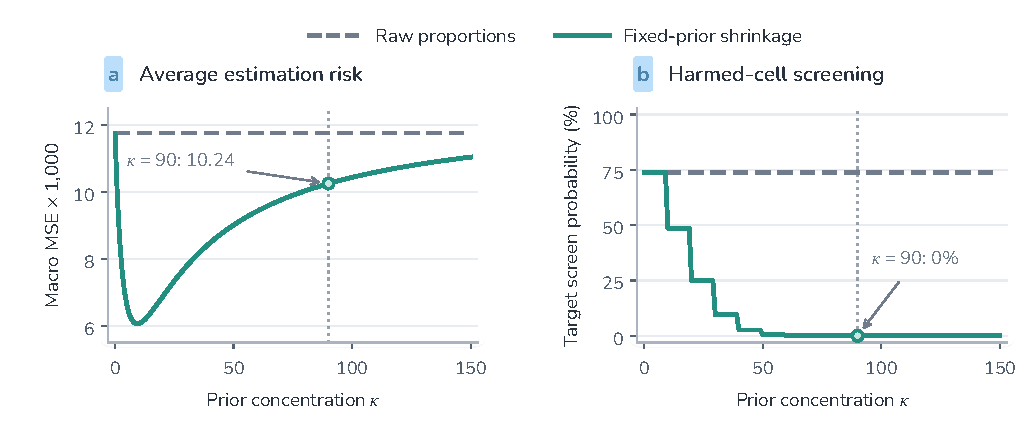
\includegraphics[width=\linewidth]{Fig1.pdf}
\caption{Fixed-prior shrinkage can reduce average risk while eliminating harmed-cell screening. Panel (a) gives macro mean squared error (MSE) over five count-ten cells, four with rate .1 and one with rate .35; panel (b) gives the exceptional-cell probability of exceeding .2 against a fixed oracle reference .1. The prior center is .1, and dotted lines mark concentration $\kappa=90$. These exact binomial threshold screens are uncalibrated and separate from unknown-complement inference}\label{fig:exact}
\end{figure*}

Comparisons of the fitted point estimates showed a similar empirical separation in specific prespecified settings (Fig.~\ref{fig:estimators}, Table~\ref{tab:estimators}). At $G=32$, $n_*=20$, and $\varepsilon=.10$, raw macro MSE was .003759, compared with .000794 for the SR point adapter and .000876 for SureMap. Nevertheless, target MSE increased from .009412 to .020410 and .019000, respectively. The raw target screen occurred in 76.7\% of the 120 repetitions, compared with 8.3\% for SR and 10.8\% for SureMap. Their screen-rate MCSEs were 3.9, 2.5, and 2.8 percentage points. The paired screen differences relative to raw were $-.6833$ (MCSE .0426) and $-.6583$ (MCSE .0435).

This finding concerns plug-in decisions and estimation objectives, not calibrated error rates. It does not demonstrate that the original SR intervals or a full SureMap uncertainty analysis miss the same proportion of harms. The behavior is also not universal across effect sizes and counts: at $n_*=80$, $\varepsilon=.30$, raw, SR, and SureMap had a target screen rate of 100\% in the 120-repeat subset, while moment EB reached 98.3\%. A zero plug-in MCSE at an all-success outcome does not establish population certainty. The control configurations and the eight real-template point comparisons remain in the reproducibility package, rather than being filtered by favorable screening behavior.

The sensitivity comparison also has a false-alert cost. In the same $G=32$, $n_*=20$, $\varepsilon=.10$ setting, the frequency of screening at least one truly nonharmful cell was 99.2\% for raw estimates, 3.3\% for SR, and 11.7\% for SureMap. These are familywise false-screen frequencies for an uncalibrated rule, not nominal-level FWER guarantees. Thus the higher raw target sensitivity does not establish a better overall decision rule. Additional point-screen diagnostics cover all seven fitted-estimator settings for these three estimators, including null and additive controls and target-risk MCSEs. This additional summary reuses retained outputs and provides no comparison of the original interval procedures.

\begin{figure*}[t]\centering
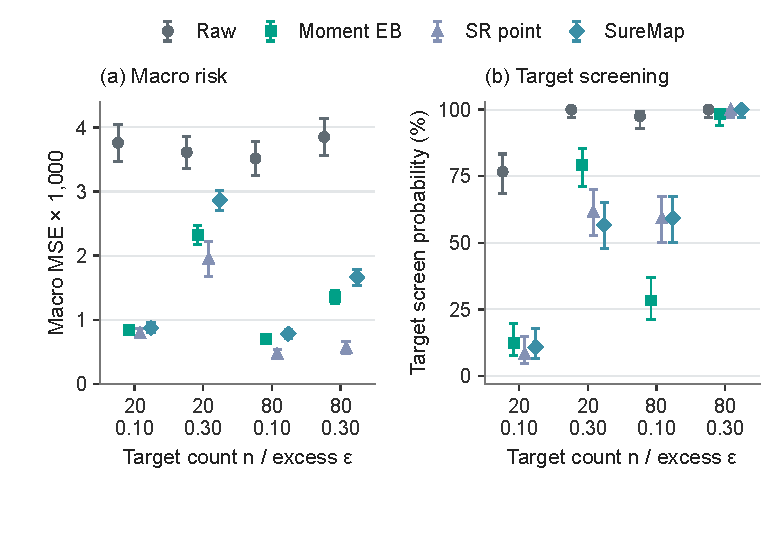
\includegraphics[width=\linewidth]{Fig2.pdf}
\caption{Lower macro risk can accompany less frequent harmed-cell screening. Four prespecified synthetic settings use $G=32$, target positive count $n$, and excess disparity $\varepsilon$ above the .05 tolerance; each tick gives $n$ above $\varepsilon$. Bars show $1.96$ Monte Carlo standard errors for mean squared error (MSE) in (a) and pointwise 95\% Wilson Monte Carlo intervals for screen probabilities in (b), from 120 paired repetitions. EB denotes empirical Bayes and SR denotes the structured-regression point adapter; the screens are uncalibrated, so panel (b) is not a frequentist power comparison}\label{fig:estimators}
\end{figure*}
% Generated by src/make_tables.py; source analysis/*.csv and retained results.
\begin{table*}[t]
\centering\small
\caption{Point-estimator diagnostics in four fixed sparse settings, based on 120 paired repetitions. Values in parentheses after MSE are Monte Carlo standard errors; brackets give pointwise 95\% Wilson intervals for simulation screen probabilities. A screen indicates that the estimated group--complement disparity exceeds .05; it is not a calibrated test. SR is the point adapter.}\label{tab:estimators}
\begin{tabular}{llrrr}
\toprule
$n_*/\varepsilon$ & Estimator & \shortstack{Macro MSE\\$\times10^3$} & \shortstack{Target MSE\\$\times10^3$} & \shortstack{Screen \%\\{[95\% MC interval]}} \\
\midrule
20/0.10 & Raw & 3.76 (0.15) & 9.41 (1.12) & 76.7 [68.3, 83.3] \\
20/0.10 & Moment EB & 0.84 (0.03) & 16.90 (0.63) & 12.5 [7.7, 19.6] \\
20/0.10 & SR point & 0.79 (0.04) & 20.41 (0.55) & 8.3 [4.6, 14.7] \\
20/0.10 & SureMap & 0.88 (0.04) & 19.00 (0.62) & 10.8 [6.4, 17.7] \\
20/0.30 & Raw & 3.61 (0.13) & 12.43 (1.69) & 100.0 [96.9, 100.0] \\
20/0.30 & Moment EB & 2.32 (0.07) & 53.44 (3.28) & 79.2 [71.1, 85.5] \\
20/0.30 & SR point & 1.95 (0.14) & 55.27 (4.76) & 61.7 [52.7, 69.9] \\
20/0.30 & SureMap & 2.86 (0.08) & 64.60 (4.23) & 56.7 [47.7, 65.2] \\
80/0.10 & Raw & 3.51 (0.14) & 2.46 (0.35) & 97.5 [92.9, 99.1] \\
80/0.10 & Moment EB & 0.70 (0.02) & 13.92 (0.66) & 28.3 [21.0, 37.0] \\
80/0.10 & SR point & 0.47 (0.03) & 9.21 (0.78) & 59.2 [50.2, 67.5] \\
80/0.10 & SureMap & 0.78 (0.03) & 8.81 (0.57) & 59.2 [50.2, 67.5] \\
80/0.30 & Raw & 3.85 (0.15) & 3.18 (0.35) & 100.0 [96.9, 100.0] \\
80/0.30 & Moment EB & 1.35 (0.05) & 18.30 (1.83) & 98.3 [94.1, 99.5] \\
80/0.30 & SR point & 0.56 (0.05) & 8.07 (0.77) & 100.0 [96.9, 100.0] \\
80/0.30 & SureMap & 1.66 (0.06) & 11.53 (1.01) & 100.0 [96.9, 100.0] \\
\bottomrule
\end{tabular}
\end{table*}


\subsection{Valid confirmation remains conservative}
Table~\ref{tab:fwer} reports the largest observed FWER for each calibrated method across the main grid. The overall maximum was .0015, or .15\%, compared with the nominal 5\% bound; full HB plus Holm reached at most .0005. These observations are compatible with the theorem but also show substantial conservatism. The finite simulations do not establish error control beyond their generating models, and common nominal levels do not mean matched realized size. In zero-event configurations, the upper endpoint of a pointwise 95\% Wilson interval with 2,000 repetitions is approximately .00192 rather than zero.

Figure~\ref{fig:power} and Table~\ref{tab:power} give target flagging behavior under the same total count budget. For $G=32$, $n_*=40$, and $\varepsilon=.20$, full HB had power .2100, versus .2585 for raw-disparity split weighting and .2510 for conflict weighting. At $n_*=160$ with the same excess, full HB reached .9140, while the split alternatives fell to .8945 and .8890. Increased evidence can therefore make retaining all data preferable to learning a testing priority. At low counts, all calibrated procedures can remain insensitive even when an uncalibrated raw screen is frequent.
% Generated by src/make_tables.py; source analysis/*.csv and retained results.
\begin{table*}[t]
\centering\small
\caption{Maximum observed familywise false-flag frequency for each method over the 60 main configurations (2,000 repeats each). The intervals are pointwise Wilson intervals for the selected configuration, not simultaneous bounds on the maximum. Nominal FWER is 5\%; the construction is conservative.}\label{tab:fwer}
\begin{tabular}{lrrrl}
\toprule
Method + Holm & Max FWER (\%) & 95\% interval (\%) & $G$ & Selected configuration \\
\midrule
Full HB & 0.050 & [0.009, 0.283] & 16 & sparse rare \\
Full H & 0.050 & [0.009, 0.283] & 16 & boundary null \\
Split uniform & 0.000 & [0.000, 0.192] & 16 & sparse rare \\
Split size & 0.000 & [0.000, 0.192] & 16 & sparse rare \\
Split raw & 0.150 & [0.051, 0.440] & 16 & boundary null \\
Split EB & 0.100 & [0.027, 0.364] & 64 & boundary null \\
Split conflict & 0.150 & [0.051, 0.440] & 64 & sparse rare \\
\bottomrule
\end{tabular}
\end{table*}

\begin{figure*}[t]\centering
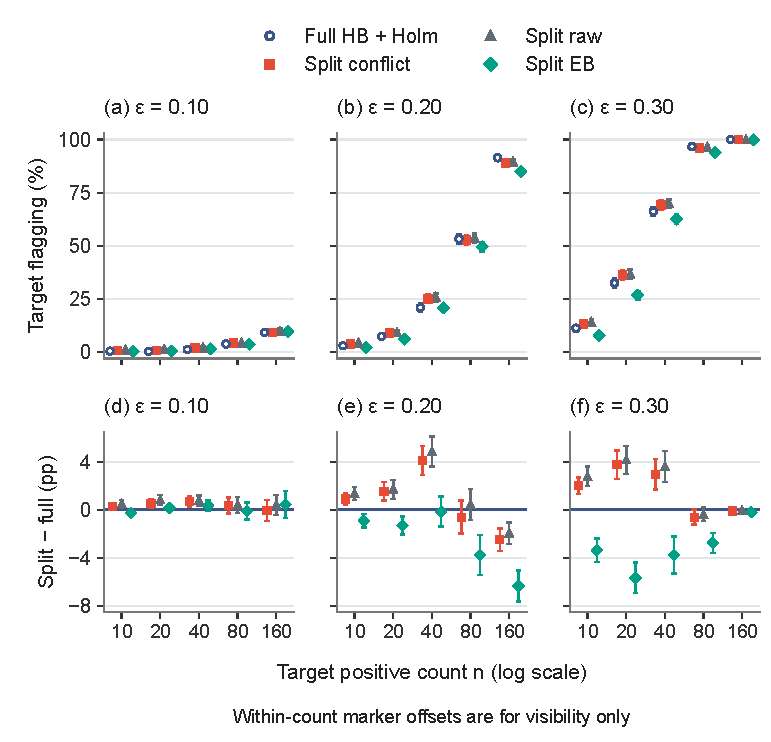
\includegraphics[width=\linewidth]{Fig3.pdf}
\caption{The value of retaining all audit data depends on target count and effect size. Panels (a--c) show absolute target flagging rates; panels (d--f) show paired split-minus-full differences in percentage points (pp), with zero indicating equal rates. Markers are offset horizontally within each nominal count for visibility. Calibrated target flagging uses $G=32$ and a common total count budget, with 2,000 repetitions per point and bars of $1.96$ Monte Carlo standard errors; difference bars use within-repetition paired contrasts. Full HB combines a Hoeffding reference bound with a binomial target tail and Holm adjustment; all split procedures use the same engine with 80\% for confirmation. EB denotes empirical Bayes. Panel effects $\varepsilon$ are true target disparity minus the .05 tolerance; the count axis is logarithmic}\label{fig:power}
\end{figure*}
% Generated by src/make_tables.py; source analysis/*.csv and retained results.
\begin{table*}[t]
\centering\small
\caption{Target flagging percentages with Monte Carlo standard errors in parentheses, for $G=32$, $\Delta=.05$, $c=.8$, and $\rho=.1$, based on 2,000 repeats. All methods use the same total generated counts and the same HB confirmation engine; the full-data method uses all observations. $\varepsilon=\delta_* -\Delta$.}\label{tab:power}
\begin{tabular}{rrrrrr}
\toprule
$n_*$ & $\varepsilon$ & Full HB & Split raw & Split EB & Split conflict \\
\midrule
20 & 0.10 & 0.40 (0.14) & 1.25 (0.25) & 0.55 (0.17) & 0.95 (0.22) \\
20 & 0.30 & 32.55 (1.05) & 36.70 (1.08) & 26.90 (0.99) & 36.30 (1.08) \\
40 & 0.20 & 21.00 (0.91) & 25.85 (0.98) & 20.85 (0.91) & 25.10 (0.97) \\
80 & 0.20 & 53.30 (1.12) & 53.75 (1.12) & 49.55 (1.12) & 52.70 (1.12) \\
160 & 0.20 & 91.40 (0.63) & 89.45 (0.69) & 85.05 (0.80) & 88.90 (0.70) \\
\bottomrule
\end{tabular}
\end{table*}


Across the 45 sparse settings, conflict weighting had a larger target flagging point estimate than full HB in 31 settings, tied in two, and lost in 12; paired differences ranged from $-.038$ to $+.065$. This summary is restricted to the fixed grid. More importantly, the additional conflict term does not improve on the simpler raw-disparity score: it lost in 43 settings and tied in two, with no wins. Its mean grid difference from raw weighting was $-.00407$, and the most negative difference was $-.0125$. These observations do not support presenting the conflict score as an improved method. Its comparison instead tests whether explicitly rewarding shrinkage disagreement contributes useful allocation information.

\subsection{Splitting and allocation must be assessed together}
The split/floor ablation in Fig.~\ref{fig:ablation} shows the cost of splitting the data. For $n_*=80$, a half-data confirmation split with floor .05 gave conflict power .330 compared with full power .536, a paired difference of $-.206$ (MCSE .0143). Changes in the floor distribute budget differently but cannot recover information that was removed from confirmation. A uniform-floor limit $\rho=1$ eliminates learned prioritization while retaining the split cost. Conversely, a small floor allows concentration on a discovered target but can divert evidence from other harmful cells. The floor protects a minimum testing budget, not a minimum detection probability.
\begin{figure*}[t]\centering
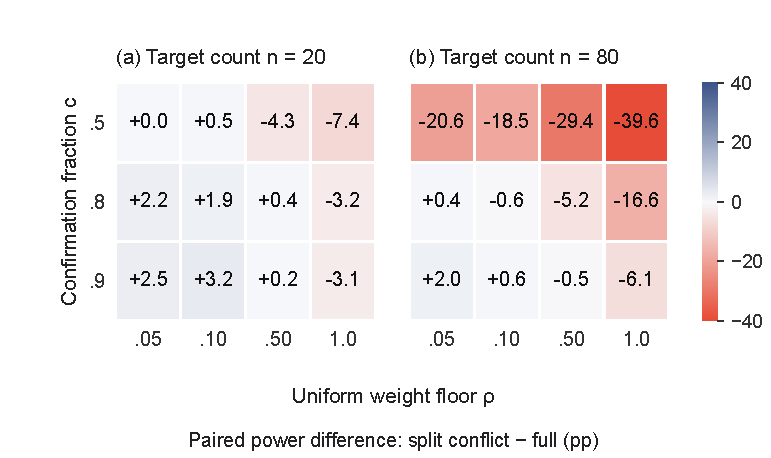
\includegraphics[width=\linewidth]{Fig4.pdf}
\caption{Large confirmation splits can reduce the power cost of conflict weighting, while small splits can incur substantial losses. Signed entries give split-conflict minus full-data HB (Hoeffding-reference/binomial-tail) power in percentage points (pp), at exceptional probability .37 and $G=32$, from 1,000 paired repetitions. The diverging scale is centered at zero, and the reference-bound parameter $\eta$ is fixed across all floors $\rho$. Companion data include paired Monte Carlo standard errors and all other scores}\label{fig:ablation}
\end{figure*}

\subsection{Real support exposes unresolved lack of information}
All original benchmark tasks contain registered cells with no audit positives (Table~\ref{tab:data}). A prior can produce a point prediction for such a cell, but cannot turn it into observed confirmation evidence. The selected real-support experiments intentionally remove unsupported cells from their testing family and change the complement weights; they cannot evaluate fairness of the omitted cells.

For the retained target cells, full HB power ranged from .020 to .034, and conflict-weighted power ranged from .030 to .058 (Fig.~\ref{fig:semi}, Table~\ref{tab:semi}). The paired gains ranged from .003 to .028. Although several differences exceeded their MCSEs, the absolute missed-harm probabilities remained high: at least .942 for conflict weighting and .966 for full HB over these configurations. We therefore interpret these experiments as evidence of sparse-support limitations, not practical recovery of rare harms. The overlap in people between the ACS tasks and the use of fixed templates further limit any cross-task generalization.
\begin{figure*}[t]\centering
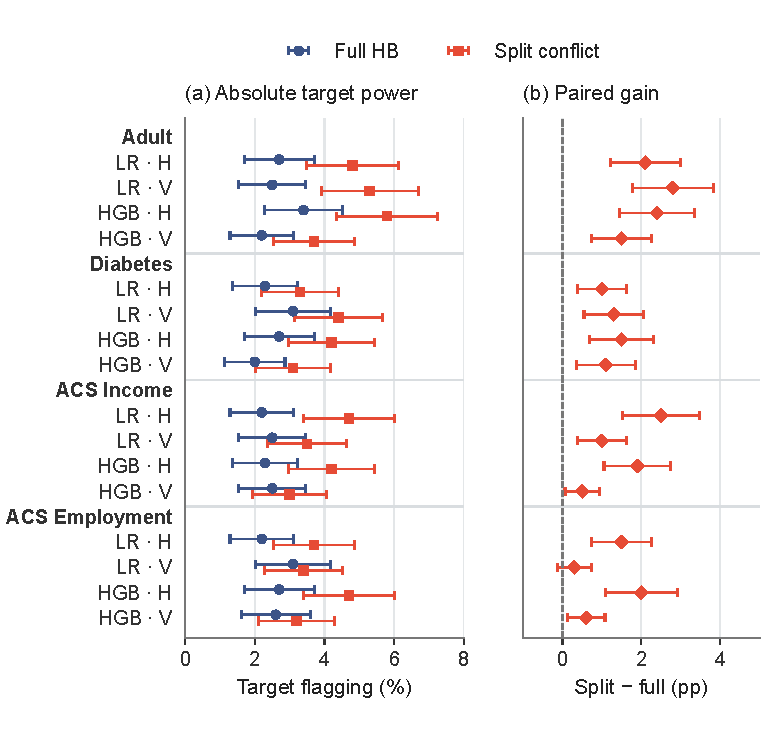
\includegraphics[width=\linewidth]{Fig5.pdf}
\caption{Modest paired gains leave absolute target power low on real-support templates. Panel (a) shows full-data HB (a Hoeffding reference bound plus a binomial target tail) and split-conflict target flagging; panel (b) shows split minus full in percentage points (pp), from 1,000 paired repetitions with bars of $1.96$ Monte Carlo standard errors, paired for differences. LR and HGB denote logistic regression and histogram gradient boosting; H and V denote homogeneous and calibration-heterogeneous baseline rates. ACS denotes the American Community Survey; all outcomes are generated with known truth on frozen supports, and every target has count ten}\label{fig:semi}
\end{figure*}
% Generated by src/make_tables.py; source analysis/*.csv and retained results.
\begin{table*}[t]
\centering\small
\caption{Known-truth real-support results: all selected target cells have $n_*=10$ and $\delta_*=.25$; 1,000 repeats. H uses homogeneous baseline rates; V uses calibration-heterogeneous templates. Differences are reported in percentage points, with paired Monte Carlo standard errors. The tested complement is defined over the selected, rounded and capped family, not the original partition.}\label{tab:semi}
\begin{tabular}{lllrrrr}
\toprule
Task & Model & Rates & $G_S$ & Full \% & Conflict \% & Difference pp \\
\midrule
Adult & LR & H & 11 & 2.7 & 4.8 & +2.1 (0.45) \\
Adult & LR & V & 11 & 2.5 & 5.3 & +2.8 (0.52) \\
Adult & HGB & H & 11 & 3.4 & 5.8 & +2.4 (0.48) \\
Adult & HGB & V & 11 & 2.2 & 3.7 & +1.5 (0.38) \\
Diabetes & LR & H & 10 & 2.3 & 3.3 & +1.0 (0.31) \\
Diabetes & LR & V & 10 & 3.1 & 4.4 & +1.3 (0.39) \\
Diabetes & HGB & H & 10 & 2.7 & 4.2 & +1.5 (0.41) \\
Diabetes & HGB & V & 10 & 2.0 & 3.1 & +1.1 (0.39) \\
ACS Income & LR & H & 10 & 2.2 & 4.7 & +2.5 (0.49) \\
ACS Income & LR & V & 10 & 2.5 & 3.5 & +1.0 (0.31) \\
ACS Income & HGB & H & 10 & 2.3 & 4.2 & +1.9 (0.43) \\
ACS Income & HGB & V & 10 & 2.5 & 3.0 & +0.5 (0.22) \\
ACS Employment & LR & H & 19 & 2.2 & 3.7 & +1.5 (0.38) \\
ACS Employment & LR & V & 19 & 3.1 & 3.4 & +0.3 (0.22) \\
ACS Employment & HGB & H & 19 & 2.7 & 4.7 & +2.0 (0.46) \\
ACS Employment & HGB & V & 19 & 2.6 & 3.2 & +0.6 (0.24) \\
\bottomrule
\end{tabular}
\end{table*}


The control-family and additional point-screen summaries are given in Tables~\ref{tab:controls} and~\ref{tab:pointcontrols}, respectively.

\subsection{Larger supported targets favor retaining confirmation data}
The 32 supplemental settings (Table~\ref{tab:support}) show a different allocation preference in larger supported cells. For target counts 130--170, full HB power ranged from .435 to .851; raw-weighted split power ranged from .407 to .778, and conflict-weighted power from .397 to .765. Raw weighting lost to full HB in all 16 larger-target configurations, with paired differences between $-.143$ and $-.014$. In contrast, the supplemental count-ten targets had full power .022--.040 and raw-weighted power .030--.059. These results preserve both the limited benefit for the smallest targets and the cost for larger targets.

For example, capped Adult LR at $n_*=140$ gave full power .802 versus raw-split .736, a paired difference of $-.066$ (MCSE .00968). Uncapped Adult LR gave .836 versus .764, a difference of $-.072$ (MCSE .00910). The capped and uncapped estimates use independently generated audit data. Because the other three tasks have identical count vectors under both cap rules, differences between their C/U point estimates are Monte Carlo variation and cannot establish a cap effect. The maximum observed FWER across all seven calibrated methods and 32 configurations was .002. The larger-target result supplies a useful supported regime for confirmation, while reinforcing that learning a priority can waste evidence. It remains conditional on the chosen cells, one injected disparity, and the transformed-family reference. The full difference-Hoeffding comparator reached power .813--.965 in these larger-target settings, exceeding full HB in all 16. Thus the confirmation engine itself can matter more than a priority score; the split-versus-full allocation comparison nevertheless keeps the HB engine identical. Both full-data engines are retained in Table~\ref{tab:support}.

\par

\subsection{Pointwise and simultaneous interval coverage differ}
The exploratory interval comparison (Table~\ref{tab:intervals}) uses the same 840 retained audit datasets. In the first setting, target coverage was 90.8\% for Wald and 95.0\% for the SAFT-style construction, while whole-family coverage was 1.7\% and 26.7\%. Their lower-endpoint tolerance rules selected the harmed target in 9.2\% and 23.3\% of repetitions and selected at least one nonharmful cell in 4.2\% and 12.5\%. These quantities concern different outputs from the original point screens and cannot be interpreted as an improvement at matched error rates. The simultaneous exact-binomial rectangle covered the target and whole family in every retained repetition, but never selected this low-support target. Across the seven settings, its target tolerance-rule frequency ranged from zero to 49.2\%, with no observed false declaration; finite simulation does not establish zero population error.

The second posterior seed did not change any target tolerance decisions in the 140 rechecked datasets. It changed three whole-family tolerance decisions among the 20 rechecked global-null datasets; the largest endpoint difference across the recheck was .0189. Thus small differences in the posterior diagnostic's false-alert frequencies are also subject to numerical Monte Carlo sensitivity. The supplement provides an interval-aware diagnostic and a classical simultaneous comparator, while leaving original SR rBLPR and Cherian--Cand\`es reproductions unresolved.

\section{Discussion and limitations}\label{sec:discussion}
The principal statistical lesson is a separation of objectives. Macro risk rewards improved estimates for many ordinary cells. A particular audit decision depends on the local bias, the effective positive count, its reference, a practical tolerance, and the budget remaining after simultaneous correction. Reporting all these quantities clarifies which conclusion the evidence supports. In particular, a lower macro MSE is not evidence that an isolated harmful group is adequately protected by a reporting threshold.

The model-mismatch interpretation needs care. A saturated design may contain the truth while the chosen penalty still attenuates a localized deviation. Conversely, a sharing structure that matches the generating rates can improve both estimation and useful screening. Our fixed-prior boundary is exact within its restricted model but elementary; it does not establish a new general impossibility theorem. The qualitative concern predates this study. The contribution is a transparent quantitative diagnostic and a reproducible comparison of its decision consequences under a matched finite-family target.

The confirmation protocol makes its assumptions explicit, at the cost of conservative inference. A worst-case heterogeneous-reference bound spends error probability on a nuisance event, and Holm protects a family rather than one selected cell. Better-calibrated inference under additional structure may have much higher power. The exploratory interval analysis adds published SAFT interval ingredients with a conditional-FNR adaptation and a classical simultaneous interval baseline. We did not compare all modern interval or simultaneous-bootstrap procedures, nor implement the original SR rBLPR confidence intervals. Consequently, the paper does not establish better inferential performance than that of SR, SAFT, or Cherian--Cand\`es auditing. Its fitted-sharing-estimator comparisons concern point estimates and uncalibrated screens. The SAFT-style tolerance rule has no claimed FWER guarantee; controlled FWER comparisons concern HB/Hoeffding and the separate exact-binomial rectangle.

Independent allocation also has a concrete limit. Raw-disparity weighting captured the principal gains in the sparse grid, while the conflict addition provided no measured gain in the primary sparse grid. The split can help some configurations and hurt others. Repeatedly tuning the score, split, or seed to maximize these results would invalidate the fixed-grid interpretation. The sufficient-bound inequality is a planning diagnostic, not an ordering of exact powers, and the available evidence supports conditional rather than uniform gains.

The finite atomic partition avoids the additional problem of searching over overlapping subgroups. The binomial target assumption requires within-cell independent, identically distributed errors in the stated design; heterogeneous targets require the separate concentration alternative. Positive counts are conditioned on and fixed. The real observational datasets contain sampling, identification, label, and dependence limitations that this conditional simulation does not resolve. ACS analyses are unweighted, the two ACS tasks overlap in people, Diabetes includes discharge-time predictors, and Adult lacks person identifiers. The generated-loss experiments remove real error dependence and filter to selected supported cells. The initial experiment fixes the target count at ten; the supplement adds selected counts 130--170 but changes cell identity and retains the same .25 disparity. This remains a restricted support-sensitivity analysis, not a broad deployment benchmark or a controlled same-cell sample-size experiment.

Finally, a statistical FNR disparity is not a complete account of harmful treatment or causal unfairness. Tolerance choice, source labels, and protected-category definitions require application judgment. The .05 tolerance is a controlled experimental choice, not a legal or ethical standard. A nonflag remains inconclusive, especially at small counts. Additional data, better domain information, and a suitable uncertainty procedure may be more useful than a more elaborate priority score.

\section{Conclusion}
We quantified a finite-sample mechanism through which sharing improves average subgroup estimation while suppressing an isolated harmful deviation in a threshold screen. Fitted SR and SureMap point estimates exhibited this separation in prespecified sparse settings, without establishing failure of their original inference procedures. Independently weighted confirmation controls false flags under the stated assumptions, but its gains depend on overcoming a data-splitting cost; the tested conflict score showed no consistent improvement over raw weighting. Sparse real-support cells retained low absolute power. An intersectional audit should therefore report estimation quality, local support, screening behavior, and calibrated evidence as separate quantities.

\ifreviewcopy\else
\section*{Acknowledgements}
OpenAI Codex assisted with literature retrieval, code development and checking, statistical derivation, analysis, figure preparation, and manuscript drafting and editing. The authors retain responsibility for the scientific claims, verification of results, and final text.
\fi

\section*{Statements and declarations}
\ifreviewcopy
\textbf{Data and code availability.} The reproducibility repository is identified in the separate title page. It contains source code, aggregate support statistics, simulated audit outcomes, and figure data. Original individual-level public datasets must be obtained from their original providers. Generated error probabilities are simulation parameters, not population ground truth.
\else
\textbf{Data and code availability.} Source code, aggregate support statistics, simulated audit outcomes, and figure data are available at \url{https://github.com/JoffinLu/Intersectional-fairness-auditing}. Original individual-level datasets must be obtained from the UCI Machine Learning Repository and the US Census Bureau using the documented acquisition scripts. Generated error probabilities are simulation parameters, not population ground truth.
\fi

\textbf{Funding.} The authors received no financial support for the research, authorship, or publication of this article.

\ifreviewcopy\else
\textbf{Author contributions.} Cenfa Lu: Conceptualization; methodology; software; formal analysis; visualization; writing -- original draft. Shuda Wu: Validation; writing -- review and editing.
\fi

\textbf{Declaration of conflicting interests.} The authors declared no potential conflicts of interest with respect to the research, authorship, or publication of this article.

\textbf{Ethical considerations.} Ethical review was not required for this study, as confirmed by the authors' institution. The study uses publicly released, de-identified secondary datasets and simulated outcomes, without participant recruitment or intervention. Original data-use conditions remain applicable.

\textbf{Consent to participate and for publication.} Not applicable to this secondary-data and simulation study; no identifiable individual records are published.

\bibliographystyle{SageH}
\begingroup
\setlength{\bibsep}{0pt}
\renewcommand{\bibfont}{\fontsize{9}{11.7pt}\selectfont}
\let\originalthebibliography\thebibliography
\def\thebibliography#1{\originalthebibliography{#1}\raggedright}
\bibliography{references}
\endgroup

\clearpage
\appendix
\section{Proofs of the finite-sample results}\label{app:theory-proofs}

The arguments below use fixed design counts. In the IID interpretation,
they apply after legitimate conditioning on the target and reference
positive counts. Independence across audit observations is assumed where
concentration is invoked. No independence between the resulting family
of p-values is required.

\subsection{Fixed-prior risk and the screening boundary}

\begin{proof}[Proof of Proposition~\ref{prop:theory-shrinkage}]
Let $v=p(1-p)$. The posterior mean has bias
$\kappa(\mu-p)/(n+\kappa)$ and variance $nv/(n+\kappa)^2$. Hence
\begin{align*}
 &R_\kappa(p)-R_0(p)\\
 &\quad=\frac{nv+\kappa^2(p-\mu)^2}{(n+\kappa)^2}-\frac vn\\
 &\quad=\frac{\kappa^2(p-\mu)^2+nv-v(n+\kappa)^2/n}{(n+\kappa)^2}\\
 &\quad=\frac{\kappa^2(p-\mu)^2-(2\kappa+\kappa^2/n)v}
 {(n+\kappa)^2},
\end{align*}
which proves Eq.~\eqref{eq:theory-risk}, including $p=0$ or $p=1$.
The strict screening event satisfies
\[
 \widetilde p>t
 \quad\Longleftrightarrow\quad
 X>nt+\kappa(t-\mu).
\]
Since $X$ takes integer values, the smallest count that passes the screen is
$\lfloor nt+\kappa(t-\mu)\rfloor+1$. This proves
Eq.~\eqref{eq:theory-cutoff}. When $t>\mu$, the real threshold increases;
the integer threshold cannot decrease but may remain unchanged. Under
Eq.~\eqref{eq:theory-collapse}, the real threshold is at least $n$, making
the strict event impossible. Conversely, if the inequality fails, $X=n$
passes; thus the condition exactly characterizes collapse of the event
over all possible counts.

If $p=t+\varepsilon$, the shrunk event is $X>np+a$ with
$a=\kappa(t-\mu)-n\varepsilon$. For $a>0$, Hoeffding's inequality gives
\[
 \begin{aligned}
 \Pr_p(A_\kappa)&\le\Pr_p(X-np\ge a)\\
 &\le e^{-2a^2/n}.
 \end{aligned}
\]
For the raw screen,
$A_0^c=\{X/n\le t\}=\{X/n-p\le-\varepsilon\}$, whose probability is at
most $e^{-2n\varepsilon^2}$. These are the bounds in
Eq.~\eqref{eq:theory-screen-bound}. If $\mu,\kappa$ were learned from
independent data, the same argument holds after conditioning on those
data, with the risk interpreted conditionally.
\end{proof}

For the constructive family, ordinary cells have $p=\mu\in(0,1)$, so
Eq.~\eqref{eq:theory-risk} is strictly negative there. The risk difference
for one exceptional cell is finite. Increasing the finite number of
ordinary cells therefore makes the macro-average difference negative,
while Eq.~\eqref{eq:theory-collapse} can still hold for the exceptional
cell. In the numerical example, the ordinary-cell raw and shrunk risks
are $0.009$ and $0.00009$. The exceptional-cell risks are $0.02275$ and
$0.0508525$. Averaging over four ordinary cells and one exceptional cell gives
$0.01175$ and $0.0102425$, respectively. The raw selection probability is
the exact tail
$1-\sum_{k=0}^2 {10\choose k}0.35^k0.65^{10-k}$, while
$nt+\kappa(t-\mu)=2+9=11$ makes the shrunk event empty.

\subsection{HB validity and standardized references}

\begin{proof}[Proof of Proposition~\ref{prop:theory-hb}]
Hoeffding's inequality for the independent, possibly heterogeneous
reference observations gives
\[
 \Pr\left\{q-\widehat q>
       \sqrt{\frac{\log(1/\eta)}{2m}}\right\}\le\eta.
\]
Clipping the endpoint at one preserves coverage because $q\le1$.
Consequently, $E_q=\{q\le U_q\}$ has probability at least $1-\eta$.
Under the null, let $\theta_0=\min\{1,q+\Delta\}$, so
$p\le\theta_0$. On $E_q$, $\theta_0\le\theta_U$. Monotone binomial
coupling implies $T_{\theta_0}(x)\le T_{\theta_U}(x)$ for every count $x$.

For completeness, $T_{\theta_0}(X)$ is super-uniform under any
$p\le\theta_0$. For any $v\in[0,1]$, the set
$\{x:T_{\theta_0}(x)\le v\}$ is empty or an upper integer tail starting at
some $k$. In the latter case,
\[
 \begin{aligned}
 \Pr_p\{T_{\theta_0}(X)\le v\}&=\Pr_p(X\ge k)\\
 &\le T_{\theta_0}(k)\le v.
 \end{aligned}
\]
This includes degenerate binomial parameters.

For $u<\eta$, $\{P_{\mathrm{HB}}\le u\}$ is empty. For
$\eta\le u<1$, clipping at one does not change this event, and
\[
 \begin{aligned}
 &\{P_{\mathrm{HB}}\le u\}\\
 &\quad\subseteq E_q^c\ \cup\
 \{T_{\theta_0}(X)\le u-\eta\}.
 \end{aligned}
\]
The union bound gives a probability of at most $\eta+(u-\eta)=u$.
The case $u=1$ is immediate. A p-value that is identically one for an unsupported
comparison is also super-uniform. This proves the proposition. The
argument does not condition the binomial law of $X$ on the random event
$E_q$. Although target/reference independence holds in the stated audit
design, this union-bound step itself requires only the binomial target
marginal and the valid reference bound.
\end{proof}

For the standardized-reference extension, write observations from cell
$h$ as $B_{hi}$, $i=1,\ldots,n_h$. Then
$\widehat q=\sum_h\sum_i(\nu_h/n_h)B_{hi}$. The sum of squared ranges is
$\sum_h n_h(\nu_h/n_h)^2=\sum_h\nu_h^2/n_h$. The weighted Hoeffding inequality therefore
gives the stated upper radius for $q=\sum_h\nu_hp_h$. The preceding proof
then applies unchanged. This argument requires $n_h>0$ whenever
$\nu_h>0$; silently discarding unsupported reference cells would change
the target and invalidate the argument.

For Eq.~\eqref{eq:theory-hoeffding}, express $d$ as a sum of independent
target observations with coefficient $1/n$ and reference observations
with coefficient $-1/m$. The sum of squared ranges is $V=1/n+1/m$.
If the difference between the average means satisfies $\delta\le\Delta$, then, for
$x>0$,
\[
 \begin{aligned}
 \Pr(d\ge\Delta+x)&\le\Pr(d-\delta\ge x)\\
 &\le e^{-2x^2/V}.
 \end{aligned}
\]
For $0<u<1$, the event $P_{\mathrm H}\le u$ implies
$d\ge\Delta+\sqrt{(V/2)\log(1/u)}$ and has probability at most $u$.
At $u=0$ it is empty, and at $u=1$ the assertion is automatic. This proves
super-uniformity for heterogeneous rates on both sides.

\subsection{Weighted Holm, the power envelope, and split cost}

\begin{proof}[Proof of Proposition~\ref{prop:theory-holm}]
Condition on the discovery data and the legitimate confirmation design. Weights
are then fixed and strictly positive. Let $I_0$ be the true-null set. If
it is empty, FWER is zero. Otherwise, let $W_0=\sum_{g\in I_0}w_g>0$.
If the procedure rejects any true null, consider the first such
hypothesis $g$ in the ordered sequence. All true nulls remain at its
testing stage. Its remaining-weight denominator $R_g$ therefore satisfies
$R_g\ge W_0$, and rejection implies
\[
 P_g\le\alpha w_g/R_g\le\alpha w_g/W_0.
\]
Taking a union over possible first true nulls and using conditional
super-uniformity gives
\[
 \begin{aligned}
 &\Pr(\text{any false flag}\mid D,\text{design})\\
 &\quad\le\sum_{g\in I_0}\frac{\alpha w_g}{W_0}=\alpha.
 \end{aligned}
\]
Each summand uses a threshold at most $\alpha\le1$. Averaging over the
conditioning variables proves strong unconditional control. The argument does not use joint
independence of p-values.

For containment, suppose $P_g/w_g\le\alpha$. All preceding ratios are at
most $\alpha$. At any such stage the remaining-weight sum is at most
one, so the Holm ratio threshold is at least $\alpha$. The procedure
reaches and rejects $g$, proving weighted-Bonferroni containment.
\end{proof}

To prove Eq.~\eqref{eq:theory-power-envelope}, again condition on
discovery and the fixed design. With $P_{\mathrm H}$, the event
$d_g\ge\Delta+b_g(w_g)$ implies $P_g\le\alpha w_g$, hence a weighted
Holm rejection. Under $\delta_g=\Delta+\varepsilon_g$ and
$\varepsilon_g>b_g(w_g)$, a lower-tail Hoeffding bound gives
\[
 \begin{aligned}
 &\Pr\{d_g<\Delta+b_g(w_g)\}\\
 &\quad\le\exp\left\{-\frac{2[\varepsilon_g-b_g(w_g)]^2}{V_g}\right\}.
 \end{aligned}
\]
Taking the complementary probability proves the envelope. Since
$w_g\ge\rho/G$, using the larger boundary $b_g(\rho/G)$ gives its
score-independent version whenever that bound is nontrivial. Neither
calculation asserts that HB has the same boundary or that a zero lower
bound implies zero actual power.

\begin{proof}[Proof of Corollary~\ref{cor:theory-split}]
Exactly proportional allocation gives $n_C=cn_A$, $m_C=cm_A$, and hence
$V_C=V_A/c$. The split and full-data sufficient boundaries satisfy
\[
 \begin{aligned}
 b_C(w_g)^2&=\frac{V_A}{2c}\log\frac1{\alpha w_g},\\
 b_A(1/G)^2&=\frac{V_A}{2}\log\frac G\alpha.
 \end{aligned}
\]
Both boundaries are nonnegative. Comparing their squares and cancelling
$V_A/2$ yields
\[
 \begin{aligned}
 &b_C(w_g)<b_A(1/G)\\
 &\quad\Longleftrightarrow\quad
 \log\frac1{\alpha w_g}<c\log\frac G\alpha\\
 &\quad\Longleftrightarrow\quad
 w_g>\alpha^{c-1}G^{-c}.
 \end{aligned}
\]
This proves the asserted equivalence solely for the specified sufficient
boundaries.
\end{proof}

\section{Reproducibility inventory}\label{app:inventory}
% Generated by src/make_tables.py; source analysis/*.csv and retained results.
\begin{table*}[t]
\centering\small
\caption{Main control families: mean flagging power across genuinely harmed cells, reported as percentages (MCSE), and the maximum observed FWER among the seven valid-flag methods in each configuration, based on 2,000 repeats. MCSE uses the per-repetition average over harmed cells. A dash indicates that there is no harmed cell. Pointwise uncertainty for every method--configuration pair is retained in the accompanying CSV.}\label{tab:controls}
\begin{tabular}{lrrrrrr}
\toprule
Control & $G$ & $|\mathcal H|$ & Full HB & Split raw & Conflict & Max FWER\% \\
\midrule
global null & 16 & 0 & -- & -- & -- & 0.10 \\
boundary null & 16 & 0 & -- & -- & -- & 0.15 \\
common harm & 16 & 1 & 97.9 (0.3) & 95.9 (0.4) & 95.2 (0.5) & 0.05 \\
dense harm & 16 & 2 & 4.2 (0.3) & 5.3 (0.4) & 5.2 (0.4) & 0.00 \\
structured additive & 16 & 1 & 0.0 (0.0) & 0.0 (0.0) & 0.0 (0.0) & 0.05 \\
global null & 32 & 0 & -- & -- & -- & 0.05 \\
boundary null & 32 & 0 & -- & -- & -- & 0.10 \\
common harm & 32 & 1 & 100.0 (0.1) & 99.7 (0.1) & 99.6 (0.1) & 0.00 \\
dense harm & 32 & 4 & 18.1 (0.4) & 18.2 (0.4) & 17.8 (0.4) & 0.00 \\
structured additive & 32 & 2 & 0.0 (0.0) & 0.0 (0.0) & 0.0 (0.0) & 0.05 \\
global null & 64 & 0 & -- & -- & -- & 0.05 \\
boundary null & 64 & 0 & -- & -- & -- & 0.10 \\
common harm & 64 & 1 & 100.0 (0.0) & 100.0 (0.1) & 99.9 (0.1) & 0.05 \\
dense harm & 64 & 8 & 29.7 (0.2) & 29.9 (0.2) & 29.5 (0.2) & 0.00 \\
structured additive & 64 & 3 & 0.0 (0.0) & 0.0 (0.0) & 0.0 (0.0) & 0.05 \\
\bottomrule
\end{tabular}
\end{table*}

\begin{table*}[t]
\centering\small
\caption{Additional point-screen diagnostics from the same 120 paired repetitions; additional summary of retained outputs. MSE columns are multiplied by $10^3$; parentheses report MCSE. Settings 1--4 are $(n_*,\varepsilon)=(20,.10),(20,.30),(80,.10),(80,.30)$; 5 is the global null, 6 is a high-count harmed target, and 7 is the additive control. The target is nonharmful in settings 5 and 7, so its screen frequency is not power. Any-null denotes the screening of at least one truly nonharmful cell; it is not an error-controlled flag. All seven estimators and per-cell false-screen summaries remain in the accompanying CSV.}\label{tab:pointcontrols}
\begin{tabular}{llrrrr}
\toprule
Setting & Estimator & Macro MSE & Target MSE & Target screen\% & Any-null\% \\
\midrule
1 & Raw & 3.76 & 9.41 (1.12) & 76.7 (3.9) & 99.2 (0.8) \\
1 & SR point & 0.79 & 20.41 (0.55) & 8.3 (2.5) & 3.3 (1.6) \\
1 & SureMap & 0.88 & 19.00 (0.62) & 10.8 (2.8) & 11.7 (2.9) \\
2 & Raw & 3.61 & 12.43 (1.69) & 100.0 (0.0) & 97.5 (1.4) \\
2 & SR point & 1.95 & 55.27 (4.76) & 61.7 (4.5) & 14.2 (3.2) \\
2 & SureMap & 2.86 & 64.60 (4.23) & 56.7 (4.5) & 53.3 (4.6) \\
3 & Raw & 3.51 & 2.46 (0.35) & 97.5 (1.4) & 100.0 (0.0) \\
3 & SR point & 0.47 & 9.21 (0.78) & 59.2 (4.5) & 5.0 (2.0) \\
3 & SureMap & 0.78 & 8.81 (0.57) & 59.2 (4.5) & 40.0 (4.5) \\
4 & Raw & 3.85 & 3.18 (0.35) & 100.0 (0.0) & 100.0 (0.0) \\
4 & SR point & 0.56 & 8.07 (0.77) & 100.0 (0.0) & 17.5 (3.5) \\
4 & SureMap & 1.66 & 11.53 (1.01) & 100.0 (0.0) & 91.7 (2.5) \\
5 & Raw & 3.99 & 9.63 (1.37) & 31.7 (4.3) & 100.0 (0.0) \\
5 & SR point & 0.14 & 0.06 (0.01) & 0.0 (0.0) & 7.5 (2.4) \\
5 & SureMap & 0.19 & 0.19 (0.04) & 0.8 (0.8) & 5.0 (2.0) \\
6 & Raw & 3.78 & 0.69 (0.09) & 100.0 (0.0) & 95.0 (2.0) \\
6 & SR point & 0.25 & 0.98 (0.11) & 100.0 (0.0) & 6.7 (2.3) \\
6 & SureMap & 0.74 & 1.62 (0.15) & 100.0 (0.0) & 23.3 (3.9) \\
7 & Raw & 4.39 & 9.60 (2.01) & 7.5 (2.4) & 100.0 (0.0) \\
7 & SR point & 0.57 & 1.53 (0.13) & 0.0 (0.0) & 31.7 (4.3) \\
7 & SureMap & 0.55 & 1.19 (0.13) & 0.0 (0.0) & 42.5 (4.5) \\
\bottomrule
\end{tabular}
\end{table*}

% Generated by src/make_tables.py; source analysis/*.csv and retained results.
\begin{table*}[t]
\centering\small
\caption{Prespecified support sensitivity with 1,000 repeats per configuration and a generated contrast of .25. HB and H are full-data engines; Raw and Conflict use split HB. C caps rounded counts at 1,000; U leaves rounded counts uncapped. Differences are reported in percentage points, with paired MCSE in parentheses. The cap changes the count vector only for Adult; C/U rows for the other tasks are independent Monte Carlo repeats of identical templates. The larger-target rule changes cell identity as well as count.}\label{tab:support}
\begin{tabular}{llrrrrrr}
\toprule
Task/model & Counts & $n_*$ & HB\% & H\% & Raw\% & Conflict\% & Raw--HB pp \\
\midrule
Adult LR & C & 10 & 3.0 & 3.0 & 5.4 & 5.2 & +2.4 (0.48) \\
Adult LR & C & 140 & 80.2 & 90.4 & 73.6 & 72.9 & -6.6 (0.97) \\
Adult LR & U & 10 & 3.6 & 3.6 & 5.9 & 5.8 & +2.3 (0.47) \\
Adult LR & U & 140 & 83.6 & 92.2 & 76.4 & 75.1 & -7.2 (0.91) \\
Adult HGB & C & 10 & 2.4 & 2.4 & 4.1 & 3.8 & +1.7 (0.46) \\
Adult HGB & C & 140 & 81.2 & 90.1 & 74.2 & 73.1 & -7.0 (0.99) \\
Adult HGB & U & 10 & 2.7 & 2.7 & 4.7 & 4.7 & +2.0 (0.44) \\
Adult HGB & U & 140 & 85.0 & 91.4 & 77.8 & 76.5 & -7.2 (0.89) \\
Diabetes LR & C & 10 & 2.5 & 2.6 & 4.5 & 4.3 & +2.0 (0.44) \\
Diabetes LR & C & 130 & 45.4 & 84.4 & 44.0 & 43.3 & -1.4 (0.99) \\
Diabetes LR & U & 10 & 2.2 & 2.5 & 3.2 & 2.9 & +1.0 (0.31) \\
Diabetes LR & U & 130 & 43.9 & 81.3 & 42.5 & 41.2 & -1.4 (1.05) \\
Diabetes HGB & C & 10 & 2.6 & 2.6 & 3.8 & 3.4 & +1.2 (0.40) \\
Diabetes HGB & C & 130 & 45.5 & 81.8 & 40.7 & 39.9 & -4.8 (0.96) \\
Diabetes HGB & U & 10 & 2.2 & 2.2 & 3.0 & 3.0 & +0.8 (0.28) \\
Diabetes HGB & U & 130 & 43.5 & 82.7 & 40.7 & 39.7 & -2.8 (1.01) \\
ACS Inc. LR & C & 10 & 2.3 & 2.3 & 4.1 & 3.8 & +1.8 (0.42) \\
ACS Inc. LR & C & 170 & 77.0 & 95.7 & 65.6 & 63.8 & -11.4 (1.05) \\
ACS Inc. LR & U & 10 & 2.8 & 2.8 & 4.0 & 4.0 & +1.2 (0.37) \\
ACS Inc. LR & U & 170 & 78.7 & 96.5 & 64.4 & 63.2 & -14.3 (1.16) \\
ACS Inc. HGB & C & 10 & 2.6 & 2.6 & 3.9 & 4.0 & +1.3 (0.36) \\
ACS Inc. HGB & C & 170 & 77.7 & 93.7 & 63.7 & 61.8 & -14.0 (1.13) \\
ACS Inc. HGB & U & 10 & 2.9 & 2.9 & 3.9 & 4.1 & +1.0 (0.37) \\
ACS Inc. HGB & U & 170 & 79.7 & 95.0 & 67.4 & 66.1 & -12.3 (1.10) \\
ACS Emp. LR & C & 10 & 2.2 & 2.1 & 3.0 & 3.1 & +0.8 (0.32) \\
ACS Emp. LR & C & 130 & 84.2 & 86.8 & 74.0 & 72.4 & -10.2 (0.98) \\
ACS Emp. LR & U & 10 & 3.4 & 3.3 & 4.1 & 4.0 & +0.7 (0.26) \\
ACS Emp. LR & U & 130 & 82.7 & 85.0 & 72.6 & 72.0 & -10.1 (0.97) \\
ACS Emp. HGB & C & 10 & 4.0 & 3.6 & 4.5 & 4.4 & +0.5 (0.26) \\
ACS Emp. HGB & C & 130 & 85.1 & 87.9 & 75.4 & 74.6 & -9.7 (0.95) \\
ACS Emp. HGB & U & 10 & 3.2 & 3.1 & 4.0 & 4.1 & +0.8 (0.32) \\
ACS Emp. HGB & U & 130 & 84.7 & 86.5 & 75.7 & 74.4 & -9.0 (0.93) \\
\bottomrule
\end{tabular}
\end{table*}

% Generated by src/make_tables.py; source analysis/*.csv and retained results.
\begin{table*}[t]
\centering\small
\caption{Exploratory interval diagnostics on the same 120 repetitions in each of the seven settings of Table~\ref{tab:pointcontrols}. Cov-T and Cov-all are target and whole-family contrast coverage; Width-T is mean target width. Rule-T and Any-null apply the rule that the lower endpoint is $>.05$, with MCSE in parentheses. Wald-P and SAFT-P use pointwise 95\% intervals; SAFT-P is the local conditional-FNR adaptation. CP-S uses a simultaneous 95\% exact-binomial rectangle. These unequal error targets do not provide a matched-FWER power comparison. Rule-T is not power for nonharmful targets (settings 5 and 7). For 0/120 and 120/120, pointwise 95\% Wilson MC intervals are [0,3.1]\% and [96.9,100]\%; complete MC intervals are retained in the CSV.}\label{tab:intervals}
\begin{tabular}{rlrrrrr}
\toprule
Setting & Interval & Cov-T\% & Cov-all\% & Width-T & Rule-T\% & Any-null\% \\
\midrule
1 & Wald-P & 90.8 & 1.7 & 0.372 & 9.2 (2.6) & 4.2 (1.8) \\
1 & SAFT-P & 95.0 & 26.7 & 0.354 & 23.3 (3.9) & 12.5 (3.0) \\
1 & CP-S & 100.0 & 100.0 & 0.756 & 0.0 (0.0) & 0.0 (0.0) \\
2 & Wald-P & 90.0 & 2.5 & 0.426 & 81.7 (3.5) & 2.5 (1.4) \\
2 & SAFT-P & 92.5 & 24.2 & 0.395 & 87.5 (3.0) & 5.0 (2.0) \\
2 & CP-S & 100.0 & 100.0 & 0.820 & 5.0 (2.0) & 0.0 (0.0) \\
3 & Wald-P & 92.5 & 1.7 & 0.193 & 45.0 (4.6) & 3.3 (1.6) \\
3 & SAFT-P & 95.8 & 23.3 & 0.190 & 53.3 (4.6) & 5.0 (2.0) \\
3 & CP-S & 100.0 & 100.0 & 0.491 & 0.0 (0.0) & 0.0 (0.0) \\
4 & Wald-P & 95.0 & 0.0 & 0.218 & 100.0 (0.0) & 7.5 (2.4) \\
4 & SAFT-P & 96.7 & 22.5 & 0.218 & 100.0 (0.0) & 10.0 (2.8) \\
4 & CP-S & 100.0 & 100.0 & 0.529 & 47.5 (4.6) & 0.0 (0.0) \\
5 & Wald-P & 72.5 & 0.0 & 0.322 & 0.0 (0.0) & 5.8 (2.1) \\
5 & SAFT-P & 96.7 & 25.0 & 0.387 & 1.7 (1.2) & 15.0 (3.3) \\
5 & CP-S & 100.0 & 100.0 & 0.814 & 0.0 (0.0) & 0.0 (0.0) \\
6 & Wald-P & 95.8 & 1.7 & 0.109 & 100.0 (0.0) & 1.7 (1.2) \\
6 & SAFT-P & 95.8 & 25.8 & 0.109 & 100.0 (0.0) & 3.3 (1.6) \\
6 & CP-S & 100.0 & 100.0 & 0.361 & 49.2 (4.6) & 0.0 (0.0) \\
7 & Wald-P & 57.5 & 4.2 & 0.262 & 0.0 (0.0) & 4.2 (1.8) \\
7 & SAFT-P & 93.3 & 21.7 & 0.365 & 0.8 (0.8) & 7.5 (2.4) \\
7 & CP-S & 100.0 & 100.0 & 0.802 & 0.0 (0.0) & 0.0 (0.0) \\
\bottomrule
\end{tabular}
\end{table*}

\textbf{SR convergence verification.} The synthetic SR runs recorded 40 convergence-warning events across the penalty search paths for 28 of 840 repetitions. Repeating the selected full-data fit for all 28 gave no convergence warnings and exactly reproduced the retained estimates; a targeted follow-up reconstructed all 28 original cross-validation paths and exactly reproduced their selected penalties, warning counts, and stored estimates. Repeating those same paths with a fixed maximum of 1,000,000 iterations and tolerance $10^{-10}$ gave no warnings and changed no selected penalty. The largest point-prediction change was $3.87\times10^{-9}$, and all seven paired-setting target screening frequencies were unchanged. This check concerns the synthetic paths that produced warnings, rather than the original ten-fold SR procedure or its intervals.

The primary files are \texttt{src/run\_simulation.py}, \texttt{src/run\_extended.py}, \texttt{src/audit\_methods.py}, and \texttt{src/prepare\_data.py}. Each scenario has an NPZ array and JSON configuration; summaries are not the only retained evidence. The principal directories are \texttt{results/main\_v1} (60 configurations, 2,000 repeats), \texttt{results/ablation\_v1} (24, 1,000), \texttt{results/newer\_baselines\_v1} (seven, 1,000; point estimators on 120), and \texttt{results/semisynthetic\_v2} (16, 1,000; point estimators on 80 in eight heterogeneous configurations). Together with the additional 32 configurations in support-sensitivity results, these runs comprise 199,000 generated audit datasets, excluding the 1,800-dataset pilot; baselines reuse subsets rather than add new audit datasets. An earlier real-support run was invalidated after an age-interval parsing error was detected in Diabetes; the error was corrected against the original records, and the run was repeated in full. Only the corrected run contributes to the results reported here.

The analysis script regenerates vector figures, paired differences and MCSEs, data-support summaries, descriptive original-group rates, and baseline failures. The complete control families, alternative scores, prevalence-weighted risks, EB concentrations, and individual weights remain in these files. Deterministic tests cover zero denominators, conditional Dirichlet means, Holm reduction, fixed-prior risks and screens, and finite heterogeneous-reference null enumerations. These checks complement, rather than replace, the mathematical assumptions and human verification.
\end{document}
